\newpage
\index{QGIS Processing Framework}
\section{QGIS Processing Framework}
\nocite{pf:www}


\begin{center}
		
\includegraphics[scale=0.30]{pictures/qgis_pf}
\end{center}

QGIS Processing Framework vznikl v rámci projektu \footnotemark{GSoC 2011} \footnotetext{Google Summer of Code. Projekt společnosti Google na podporu studentu. více na http://code.google.com/soc/}. Student Camilo Polymeris z univerzity Universidad de Concepción si kladl za cíl napsat obecný framework, do kterého budou zapadat všechny moduly všech pluginů QGISu a každý modul bude možné použít buď samostatně nebo spojovat s jinými.

V době psaní této práce byla na světě první verze Processing Frameworku a vše nasvědčovalo tomu, že práce na frameworku budou pokračovat a nástroje v Processing Frameworku budou přibývat. Existovala totiž pouze částečná  podpora pro funkce z SAGA GIS a plugin zpřístupňující funkce \index{Orfeo Toolbox, OTB} Orfeo Toolboxu (OTB). Orfeo Toolbox je svobodný software poskytující nástroje pro zpracování snímku z \index{DPZ, dálkový průzkum Země} dálkového průzkumu Země.

V době mého připojení k QGIS Processing Frameworku byl projekt na začátku. Pro seznámení s projektem jsem přepsal Processing Manager (toolbox) z QTreeWidget do MVC architektury.

\begin{figure}[h]
	\centering
	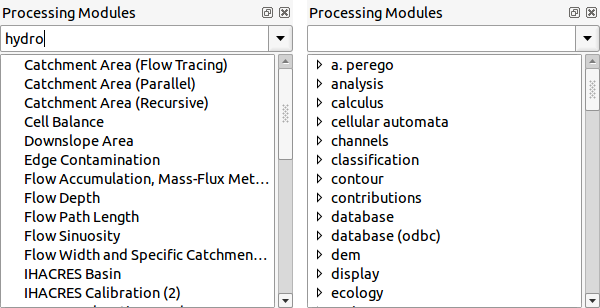
\includegraphics[scale=0.5]{pictures/pf/processing_manager_small}
	\caption{QGIS Processing Framework - Processing Manager}
  	\label{pf:pm}
\end{figure}

Processing Manager je část QGIS Processing Frameworku, která zpřístupňuje všechny moduly dostupné skrze QGIS Processing Framework z jednoho místa. Jedná se o panel se seznamem modulů, které jsou rozděleny podle tagů do různých skupin (například 'raster', 'hydrology'). Každý modul obsahuje seznam tagů, které napovídají, k čemu daný modul slouží. Uživatel může najít hledaný modul prohledáváním samotného stromu, či využít vyhledávací okénko v horní části panelu. Processing Manager prohledává tagy daného modulu a jeho název. Modul obsahuje dále popis, ale protože se tagy generují z tohoto popisu, není nutné popis procházet \figurename \ref{pf:pm}.

Modul je reprezentován třídou \textbf{Module} a jeho instance třídou \textbf{ModuleInstace}. Z třídy \textbf{Module} získáváme informace o modulu. Pomocí metody $name$() získáme jméno modulu, metoda $description$() vrací popis, metoda $tags$() a metoda $instance$() vrací instanci třídy \textbf{ModuleInstace} daného modulu. Zavoláním metody $parameters$() získáme seznam parametrů daného modulu. Parametry jsou třídy \textbf{Parameter}.

U \textbf{ModuleInstace} můžeme pomocí metody $setValue$(Parameter, hodnota) přiřazovat parametrům konkrétní hodnoty. Metodou $value$(Paramter) získáme hodnotu parametru. Pomocí metody $setState$() s parametrem "2" spouštíme daný modul. Metoda $module$() vrací module (Module).

Parametry jsou třídy \textbf{Parameter}. Uchovávají v sobě informaci o názvu a popisu parametru, zdali je parametr povinný, jakého je typu a role (např. vstupní, výstupní) a jeho defaultní hodnotu. Přehled metod třídy \textbf{Parameter} je zobrazen v [\tablename \ref{tab:metPar}].

\begin{table}[!]
	\centering
	\begin{tabular}{|c|c|}
	\hline
	metoda & popis \\
	\hline
	\hline
	name() & vrací jméno\\
	description() & vrací popis\\
	type() & vrací typ [viz Tabulka \ref{tab:pf_parametry} \\
	setRole(role) & nastaví roli\\
	role() & vrací roli\\
	setMandatory(bool) & nastaví zdali je parametr povinný\\
	isMandatory() & vrátí hodnotu, zdali je parametr povinný\\
	setDefaultValue() & nastaví defaultní hodnotu parametru\\
	defaultValue() & vrátí defaultní hodnotu parametru \\
	\hline
	\end{tabular}
	\caption{Metody třídy Parameter.}
	\label{tab:metPar}
\end{table}

Modulů z \textbf{QGIS Processing Framework} jsou přístupné buď přes \textbf{Processing Manager} nebo přes pythoní konzoli [\autoref{pf:konzole}]. Konzoli lze spustit například klávesovou zkratkou \textbf{Ctrl+Alt+ p}. 
\newpage

\begin{lstlisting}[label=pf:konzole,caption={Přístup k modulům přes konzoli.}] 
import processing

# seznam vsech registrovanych modulu
processing.framework.modules()
	
# vrati dany modulu
mod = processing.framework['nazev_modulu']
# vraci seznam parametru daneho modulu
mod.parameters()

# vytvori instanci modulu
instance = mod.instance()
# nastavi paramter
instance.setValue(parametr, hodnota)
# spusti modul
instance.setState(2)

# ziskani hodnoty parametru
instance.value(parametr2)
\end{lstlisting}

Spouští-li se modul přes \textbf{Processing Manager}, objeví se dialogové okno pro nastavení parametrů modulu a následné spuštění [viz \figurename \ref{pf:dialog}].

\begin{figure}[!]
	\centering
	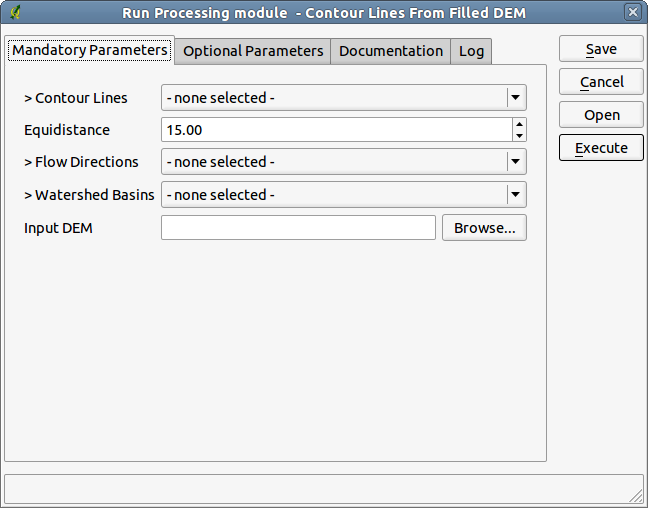
\includegraphics[scale=0.5]{pictures/pf/processing_dialog}
	\caption{QGIS Processing Framework - okno pro nastavení a spuštění modulu}
  	\label{pf:dialog}
\end{figure}

%%%%%%%%%%%%%%%%%%%
%%% SAGA Plugin %%%
%%%%%%%%%%%%%%%%%%%
\newpage
\subsection{SAGA Plugin}
SAGA Plugin vznikl v rámci stejného projektu Camila Polymeris pro GSoC 2011. Měl zpřístupňovat funkce programu SAGA GIS pomocí jeho API uživatelům Quantum GIS. Na stránkách projektu \cite{pf:supportedModules} se deklaruje, že by mělo být podporováno 170 modulů z celkových 425. Toto číslo vychází z předpokladu, že moduly, u kterých jsou všechny vstupní i výstupní parametry podporovány, pracují správně. Podporované parametry SAGA GIS a jejich reprezentace v Processing Frameworku \ref{tab:saga_parameters}. Parametry SAGA GIS, které nejsou podporované Processing Frameworkem$:$ \textit{Table field, Data Object, Grid list, Table, Node, Shape list, Parameters, Point Cloud, TIN, Static table, Table list, Color, TIN list a Colors}. Dále nejsou podporované interaktivní moduly. Bohužel ale nebyl plugin plně dokončen a skutečný počet správně pracujících pluginů není roven 170. \\

\begin{table}[h]
	\centering
	\begin{tabular}{|c|c|}
		\hline
		\textbf{SAGA parametr} & \textbf{PF Parameter} \\
		\hline
		\hline
		Int & \multirow{3}{*}{NumericParameter}\\
		Double & \\
		Degree & \\
		\hline				
		Range & RangeParameter\\	
		\hline
		Bool & BooleanParameter\\		
		\hline
		String & \multirow{2}{*}{StringParameter}\\
		Text & \\
		\hline
		Chioce & ChoiceParameter\\
		\hline
		FilePath & PathParameter\\
		\hline
		Shapes & VectorLayerParameter\\
		\hline
		Grid & RasterLayerParameter\\		
		\hline	
	\end{tabular}
	\caption{parametry SAGA GIS podporované Processing Frameworkem}
	\label{tab:saga_parameters}
\end{table}


%%%%%%%%%%%%%%%%%%%%%%%%%%%%
%%% Psaní pluginu pro PF %%%
%%%%%%%%%%%%%%%%%%%%%%%%%%%%

\subsection{Psaní pluginu pro PF}
Plugin pro QGIS Processing Framework se v mnohém neliší od normálních pluginů psaných pro QGIS. Inicializační soubor se prakticky vůbec neliší. Třída reprezentující samotný plugin obsahuje navíc metodu \textit{modules}(), která vrací seznam modulů třídy processing.\textbf{Module} (dále jen Module), který poskytuje daný plugin. Plugin samotný se musí registrovat v frameworku. To se provede příkazem \begin{scriptsize}processing.framework.registerModuleProvider(self)\end{scriptsize}, který se vloží do metody \textit{initGUI}().

Plugin tedy může obsahovat několik modulů, které vrací pomocí metody \textit{modules}(). Každý modul se skládá ze sebe a ze svojí "instance". Tedy z podtříd tříd Module a processing.ModuleInstance (dále jen ModuleInstance). Module je pro daný modul základní třída, která definuje typy parametry modulu, jeho název, popis a tagy. A vrací jeho instanci v podobě ModuleInstance, která slouží ke spouštění modulu s nastavenými parametry a spravuje, co se děje po provedení modulu. To znamená, že pakliže chceme spustit modul, musíme nastavit parametry a ty se nastavují v instanci, ne v modulu samotném. Modul poté spustíme metodou instance setStatus(2). Instance by mela obsahovat kód, který vstupní parametry zpracuje a poté také nastaví výstupní hodnoty.

Modul může mít několik vstupních a výstupních parametrů. V současné době dovoluje framework uživateli použít parametry \ref{tab:pf_parametry}.

\begin{table}	
	\centering
	\begin{tabular}{|c|c|c|}
		\hline
		\textbf{parametr} & \textbf{popis} & \textbf{grafická reprezentace}\\
		\hline
		\hline
		NumericParameter & číslo & QSpinBox\\
		\hline
		RangeParameter & dvojice číselných hodnot & pár QSpinBox\\	
		\hline
		BooleanParameter & boolean & QCheckBox\\		
		\hline
		\multirow{2}{*}{ChoiceParameter} & seznam možností & \multirow{2}{*}{QComboBox}\\
		& např. vrstev, metod & \\
		\hline
		StringParameter & textový řetězec & QLineEdit \\
		\hline
		PathParameter & cesta k souboru & QLineEdit + QPushButton \\
		\hline
		\multirow{2}{*}{VectorLayerParameter} & \multirow{2}{*}{QgsVectorLayer} & QComboBox s registrovanými \\
		& & vektorovými vrstvami\\
		\hline
		\multirow{2}{*}{RasterLayerParameter} & \multirow{2}{*}{QgsRasterLayer} & QComboBox s registrovanými \\
		& & rastrovými vrstvami\\		
		\hline	
	\end{tabular}
	\caption{parametry podporované Processing Frameworkem}
	\label{tab:pf_parametry}
\end{table}

Jako příklad uvedeme plugin Plugin, který bude mít na vstupu dva parametry. Jeden parametr pro načtení cesty k rastrovému souboru a druhý pro zadání jeho názvu, pod kterým se objeví v QGISu. Výstup bude jeden - rastr třídy QgsRasterMapLayer. Příklad je pouze ilustrativní.

Inicializační soubor nebudu uvádět, protože se nijak neliší od toho, když píšeme normální plugin pro QGIS. Soubor se samotným pluginem bude obsahovat třídu Plugin, která reprezentuje náš plugin [\autoref{pf:plugin}]. Dále třídu RasterToQgis(processing.Module) [\autoref{pf:rasterToQgis}] a třídu RasterToQgisInstance(processing.ModuleInstance) [\autoref{pf:rasterToQgisInstance}] .\\

\newpage
\begin{lstlisting}[caption={Třída Plugin pro QGIS Processing Framework}, label=pf:plugin, morekeywords={Plugin, __init__, modules, initGUI, unload}]
class Plugin:
    def __init__(self, iface):
        self.iface = iface
    def unload(self):
        pass
    def modules(self):
        return [self.rasterInputLayer]
    def initGui(self):
        self.rasterInputLayer = RasterToQgis(self.iface)
        processing.framework.registerModuleProvider(self)
\end{lstlisting}
\newpage
\begin{lstlisting}[caption={Třída RasterToQgis reprezentující modul pro QGIS Processing Framework}, label=pf:rasterToQgis, morekeywords={processing.Module,RasterToQgis, __init__, instance, RasterToQgisInstance, PathParameter, StringParameter, RasterLayerParameter}]
class RasterToQgis(processing.Module):
    def __init__(self, iface = None):
        self.iface = iface
        self.inParamPath = PathParameter("Path to input raster",
        	role=Parameter.Role.input)
        self.inParamName = StringParameter("Name of layerr",
        	role=Parameter.Role.input)
        self.outParam = RasterLayerParameter("Output raster",
        	role = Parameter.Role.output)
        self.outParam.setMandatory(False)
        processing.Module.__init__(self, "Input raster by path", 
            description = "Description",
            parameters = [self.inParamPath,self.inParamName,self.outParam], 
            tags = ["raster", "input"])

    def instance(self):
        return RasterToQgisInstance(self, self.inParamPath,
        							self.inParamName,  self.outParam)
\end{lstlisting}

V příkladu [\autoref{pf:rasterToQgis}] jsme u parametrů jsem nastavili pouze nejnutnější atributy jako název a roli. Role nám říká, zdali je parametr povinný či volitelný. U parametrů můžeme nastavit také popis či počáteční hodnotu při jejich tvorbě pomocí parametrů v konstruktoru \textit{description} a \textit{defaultValue}. Nastavit defaultní hodnotu můžeme také metodou \textit{setDefaultValue}(value). \\

\begin{lstlisting}[caption={Třída RasterToQgisInstance reprezentující instanci modulu pro QGIS Processing Framework}, label=pf:rasterToQgisInstance, morekeywords={processing.ModuleInstance, RasterToQgisInstance, __init__, valueChangedSignal,onStateParameterChanged, QgsRasterLayer,setValue }]
class RasterToQgisInstance(processing.ModuleInstance):
    def __init__(self, module, inParamPath, inParamName,  outParam):
        self.inParamPath = inParamPath
        self.inParamName = inParamName
        self.outParam = outParam
        processing.ModuleInstance.__init__(self, module)
        QObject.connect(self,
            self.valueChangedSignal(self.stateParameter),
            self.onStateParameterChanged)
    def onStateParameterChanged(self, state):
        if state == StateParameter.State.running:            
            path = self[self.inParamPath]
            name = self[self.inParamName]
            raster = QgsRasterLayer(path, name)
            self.setValue(self.outParam, raster)
            self.setState(StateParameter.State.stopped)
\end{lstlisting}

Instance kontroluje stav (state) modulu. Je-li nastaven hodnotu 2 (StateParameter.State.running) vezme si vstupní parametry a na jejich základě vytvoří novou rastrovou vrstvu \textbf{QgsRasterLayer}. A tu nastaví do odpovídajícího výstupního parametru.

%%%%%%%%%%%%%%%%%%
%%% Conclusion %%%
%%%%%%%%%%%%%%%%%%

\subsection{Závěr}

Bylo by dobré vyřešit vstupní vrstvy aby například rastrová vrstva zadaná jako PathParameter byla kompatibilní s parametrem RasterLayerParameter. Dát vývojáři pluginu možnost, aby mohl  uživatel zadat vrstvu buď pomocí cesty nebo výběrem z již načtených vrstev. Dát tedy uživateli obě možnosti.

Do této chvíle je napsán OTB Plugin pro zpracování družicových snímků a rozepsán SAGA Plugin s podporou několika pluginů z SAGA GIS.

Camilo Polymeris měl v plánu pokračovat na projektu v rámci GSoC 2012, ale po objevení frameworku SEXTANTE svoji žádost stáhl a zapojil se do prací na SEXTANTE. QGIS Processing Framework se tedy zdá být mrtvým projektem.

Dále bych chtěl upozornit, že během vývoje se změnila struktura dat. Na začátku bylo jádro frameworku uloženo v \begin{scriptsize}python/processing\end{scriptsize} a Processing Manager, GUI a dialog pro spouštění modulů v \begin{scriptsize}python/plugins/processingplugin\end{scriptsize}. V současné době je vše uloženo v \begin{scriptsize}python/processingmanager\end{scriptsize}, resp. jádro v \begin{scriptsize}python/processingmanager/processing\end{scriptsize}. To může na začátku psaní vlastního pluginu způsobit menší problém v chybně zadané cestě k frameworku.

\newpage
